%% General Java-focused CV - Álvaro López Álvarez (English)
%% Generic CV for Java / Spring Boot backend roles. Synced with main_java_es.tex.
%% Compile with: lualatex main_java_en.tex
%% (pdflatex often fails on modern MiKTeX with fontawesome5 font-expansion errors.)

\documentclass[11pt,a4paper,sans]{moderncv}
\moderncvstyle{banking}
\moderncvcolor{blue}

% Force both first and last name AND section headings to render in moderncv
% blue (color1). Default banking on lualatex+MiKTeX leaves these black, which
% looks inconsistent with the rest of the blue accent scheme.
\renewcommand*{\firstnamestyle}[1]{{\fontsize{34}{36}\bfseries\upshape\color{color1}#1}}
\renewcommand*{\lastnamestyle}[1]{{\fontsize{34}{36}\bfseries\upshape\color{color1}#1}}
\renewcommand*{\sectionstyle}[1]{{\sectionfont\color{color1}#1}}

\usepackage[utf8]{inputenc}
\usepackage{needspace}
\usepackage{hyperref}
\hypersetup{
    colorlinks=true,
    linkcolor=blue,
    filecolor=magenta,
    urlcolor=blue,
    pdftitle={Álvaro López Álvarez - CV},
    pdfpagemode=FullScreen,
}
\usepackage[scale=0.80]{geometry}
\usepackage{import}
\usepackage{eso-pic}

% personal data
\name{Álvaro}{López Álvarez}
\address{Valencia, España}{}{}
\phone[mobile]{+34 640764553}
\email{alvaro.lopez.dev@gmail.com}
\extrainfo{\href{https://www.linkedin.com/in/alvarolopez-dev}{LinkedIn}, \href{https://github.com/alerone}{GitHub}, \href{https://alerone.github.io/portfolio}{Portfolio}}

% moderncv's banking style (head variant 3) does not wire up \photo at all -
% it is silently ignored. Overlay the photo directly instead, anchored to the
% page corner so it is independent of the centered banking header layout.
\AddToShipoutPictureFG{%
  \ifnum\value{page}=1
    \AtPageUpperLeft{%
      \hspace*{\dimexpr\paperwidth-2.3cm-1.3cm\relax}%
      \raisebox{\dimexpr-1.3cm-2.3cm\relax}{\fboxsep0pt\fboxrule0.6pt\fcolorbox{color1}{white}{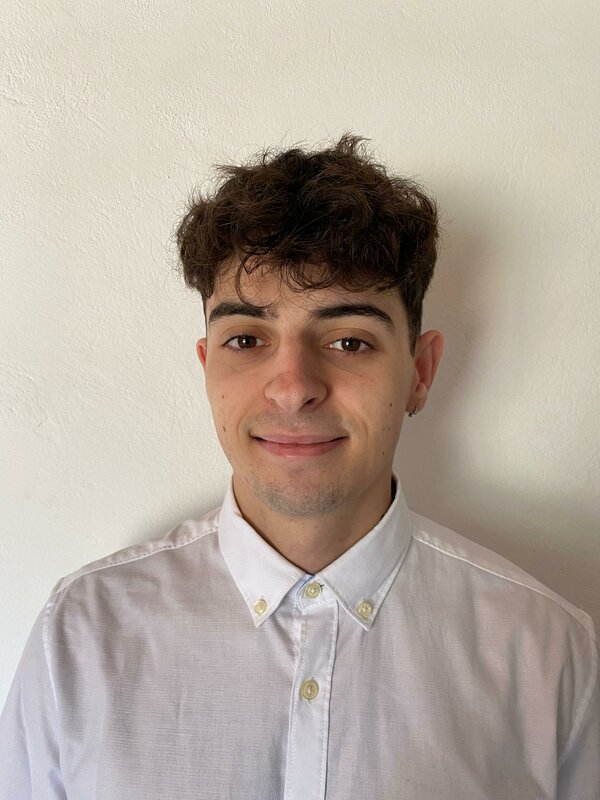
\includegraphics[width=2.3cm]{photo}}}%
    }%
  \fi
}

\begin{document}

\makecvtitle

% Headline: what the candidate is / is aiming for, visible at first glance.
\vspace{-4pt}
\begin{center}
{\Large\bfseries\color{color1}Junior Backend Developer \textbar{} Java \& Spring Boot}\\[3pt]
{\normalsize\color{color2}REST APIs \textbullet{} Event-Driven Microservices \textbullet{} Hexagonal Architecture}
\end{center}

% ============================================================
%     PROFILE STATEMENT
% ============================================================

\vspace{2pt}
\small{\textbf{Software engineer specializing in the Java ecosystem}, building REST APIs and event-driven microservices with clean, testable architecture. Hands-on Spring Boot 3 work includes Kafka-based microservices (outbox pattern, dead-letter topics, idempotent processing), REST APIs with JPA and Jakarta Validation, and integration testing with Testcontainers. Currently deepening my Java skills through self-study of hexagonal architecture (ports \& adapters) with Spring Boot and architectural design patterns. Also proficient in Golang, TypeScript and React, with professional R\&D experience building LLM-based agents at ITI. Master's Degree in Computer Engineering (final grade 8.8/10) and certified B2 English.}

% ============================================================
%     CORE COMPETENCIES
% ============================================================

\section{Core Competencies}
\vspace{1pt}
\begin{itemize}

\item \textbf{Java Backend}: Java, Spring Boot 3, Spring Data JPA, Jakarta Validation, REST APIs, DTOs/mappers, centralized error handling, JUnit, Testcontainers

\item \textbf{Architecture}: Hexagonal architecture (ports \& adapters), event-driven microservices, outbox pattern, dead-letter topics, idempotent consumers

\item \textbf{Messaging \& Infrastructure}: Apache Kafka, NATS, Docker, Docker Compose, Apache APISIX, PostgreSQL

\item \textbf{Other Languages \& Frontend}: Golang, TypeScript/JavaScript, React, Python, Kotlin, SQL

\item \textbf{LLM/AI Engineering}: LangChain, LangGraph, Gemini API, OpenAI API, RAG pipelines

\item \textbf{Tools \& Practices}: Git, GitHub Actions, TDD, OAuth 2.0/JWT, Firebase, Supabase, Vercel, Render, NeoVim

\end{itemize}

% ============================================================
%     PROFESSIONAL EXPERIENCE
% ============================================================

\section{Professional Experience}
\vspace{3pt}
\begin{itemize}

% --- Most Recent Role ---
\needspace{5\baselineskip}
\item{\cventry{Feb 2026--Jun 2026}{R\&D Developer}{Instituto Tecnológico de Informática (ITI)}{Valencia, España}{}{\vspace{1pt}
\begin{itemize}
    \item Implemented LLM-based improvements to a search engine
    \item Built a LangGraph multi-step agent that converts natural-language questions into validated, read-only SQL queries to resolve data-access policies over a PostgreSQL data-governance schema
    \item Applied safety-conscious agentic design: schema/table selection, structured SQL generation, execution validation, retry-on-error
    \item Worked within an application focused on management, governance, and sovereignty of industrial data
\end{itemize}}}

\vspace{3pt}

% --- Previous Role ---
\needspace{5\baselineskip}
\item{\cventry{Feb 2024--Jun 2024}{Full-Stack Developer Intern}{Instituto Tecnológico de Informática (ITI)}{Valencia, España}{}{\vspace{1pt}
\begin{itemize}
    \item Developed and maintained the corporate personnel management application (Intranet)
    \item Implemented new frontend features using React and TypeScript, improving internal usability
    \item Contributed to backend development, ensuring smooth integration between services
\end{itemize}}}

\end{itemize}

% ============================================================
%     SELECTED JAVA PROJECTS
% ============================================================

\section{Selected Java Projects}
\vspace{1pt}
\begin{itemize}

\item \textbf{Kafka + Spring Boot Ticketing Platform} -- \textit{Java, Spring Boot 3, Apache Kafka, Testcontainers}: Event-driven microservices (reservation, payment, notification, audit) using the outbox pattern, dead-letter topics, idempotent processing, and integration tests with Testcontainers.

\item \textbf{English Learning API} -- \textit{Java, Spring Boot, Spring Data JPA, Jakarta Validation}: REST API for practicing English phrasal verbs and collocations. JPA entities, DTOs and mappers, request validation, centralized error handling, and randomized practice challenges with attempt tracking.

\item \textbf{HTTP Server from TCP (Java)} -- \textit{Java, JUnit}: HTTP/1.1 server implemented directly on raw sockets with no framework, built to deepen Java fundamentals: I/O streams, concurrency with executors, and unit testing with JUnit.

\end{itemize}

% ============================================================
%     OTHER PROJECTS
% ============================================================

\section{Other Projects}
\vspace{1pt}
\begin{itemize}

\item \textbf{FaaS with Golang} -- \textit{Go, Docker, NATS JetStream, Apache APISIX}: Distributed Function-as-a-Service platform where workers execute arbitrary Docker-image functions. NATS JetStream work-queues, APISIX gateway for JWT auth and rate limiting, horizontal scaling via Docker Compose replicas.

\item \textbf{AIDucate} -- \textit{Go, Gin, PostgreSQL, React, TypeScript, Gemini API}: AI-powered SaaS platform generating personalized study plans and exercises. JWT-authenticated backend with PostgreSQL; React frontend on Vercel, backend on Render. \textit{(In progress)}

\item \textbf{ValenMove} -- \textit{Kotlin, MVVM, JSoup}: Native Android app unifying Valencia's public transport (EMT, Metrovalencia, Valenbisi) with real-time arrivals from reverse-engineered public APIs and Open Data. Final Degree Project, grade 9/10.

\end{itemize}

% ============================================================
%     CONTINUOUS LEARNING
% ============================================================

\section{Continuous Learning}
\vspace{1pt}
\begin{itemize}
\item \textbf{Hexagonal Architecture in Java with Spring Boot} -- self-study (in progress): ports \& adapters, framework-independent domain, Spring Boot adapters.
\item \textbf{Architectural Design Patterns} -- self-study (in progress): software architecture patterns and their trade-offs.
\end{itemize}

% ============================================================
%     EDUCATION
% ============================================================

\section{Education}
\vspace{1pt}
\begin{itemize}

\needspace{5\baselineskip}
\item{\cventry{2024--2026}{Master's Degree in Computer Engineering (MUIINF)}{Polytechnic University of Valencia (UPV)}{Valencia, España}{}{\vspace{1pt}
Completed (Sep 2026), final grade 8.8/10. Topics: distributed systems, high-performance computing, cybersecurity, embedded systems.
}}

\vspace{3pt}

\needspace{5\baselineskip}
\item{\cventry{2020--2024}{Grado (BSc) in Ingeniería Informática, Software Engineering track}{Polytechnic University of Valencia (UPV)}{Valencia, España}{}{\vspace{1pt}
GPA: 8.88/10. Thesis (TFG): ``ValenMove -- Unified Public Transport App'' (grade 9/10).
}}

\end{itemize}

% ============================================================
%     LANGUAGES
% ============================================================

\section{Languages}
\vspace{1pt}
\begin{itemize}
\item Spanish (native), Catalan (native), English (certified B2, confident conversational).
\end{itemize}

% ============================================================
%     REFERENCES
% ============================================================

\section{References}
\vspace{1pt}
\begin{itemize}
\item{Available upon request.}
\end{itemize}

\end{document}
